\documentclass[conference]{IEEEtran}
\IEEEoverridecommandlockouts
% The preceding line is only needed to identify funding in the first footnote. If that is unneeded, please comment it out.
\usepackage{cite}
\usepackage{amsmath,amssymb,amsfonts}
\usepackage{algorithmic}
\usepackage{graphicx}
\usepackage{textcomp}
\usepackage{xcolor}
\usepackage{matlab-prettifier}
\usepackage[]{geometry}
\usepackage{graphics}
\def\BibTeX{{\rm B\kern-.05em{\sc i\kern-.025em b}\kern-.08em
    T\kern-.1667em\lower.7ex\hbox{E}\kern-.125emX}}
\begin{document}

\title{Matlab Basics for Polynomial, Laplace and Transfer Function*\\
{\footnotesize \textsuperscript{}Lab Report: 01}
{\footnotesize \textsuperscript{} Course Code: EEE4706}
\thanks{Identify applicable funding agency here. If none, delete this.}
}

\author{\IEEEauthorblockN{ Mohammad Zakaria}
\IEEEauthorblockA{\textit{Dept. of EEE} \\
\textit{International Islamic University Chittagong}\\
ET193025 \\
zakaria.eee.iiuc@gmail.com}\\+8801715678738

}

\maketitle

\begin{abstract}
Matlab is a programming language and environment that is widely used in the engineering and scientific communities for tasks such as polynomial and function fitting, signal processing, and control systems analysis. The Laplace transform and transfer function are mathematical tools that are commonly used in these fields. Matlab includes built-in functions and toolboxes for working with polynomials, Laplace transforms, and transfer functions, making it a powerful tool for these types of analysis. In MATLAB, a polynomial is represented by a row vector. Only the coefficients of the polynomials are entered through keyboard. 


\end{abstract}

\begin{IEEEkeywords}
polynomial, laplace transform, transfer function
\end{IEEEkeywords}

\section{Introduction}
Matlab provides functions for polynomial fitting, roots of polynomials, and polynomial manipulation, among other things. The Laplace transform is a widely used tool in signal processing, control systems, and other fields, and Matlab provides built-in functions for computing the Laplace transform of functions, as well as for manipulating and analyzing signals in the frequency domain. Transfer function is a mathematical representation of a linear time-invariant system, and Matlab can be used to compute and analyze transfer functions, as well as to design and simulate control systems.

In summary, Matlab can be used for polynomial, Laplace transform and transfer function analysis by providing built-in functions, toolboxes and visualization options, which makes it a powerful tool for these types of analysis.

\section{Objectives:}

\subsection{The objectives of this lab is:}

\begin{itemize}
    \item  Handling Polynomial In MATLAB.
    \item Laplace Transform 
    using MATLAB.
    \item Transfer Function and pole zero map.
    \item  Response of a system through Transfer Function.
\end{itemize}
 


\section{Command Description}
\subsection{Handling Polynomials in MATLAB}
\subsubsection{Polynomial Representation:}
A polynomial in MATLAB is represented 
by a row vector. Only the polynomial 
coefficients are input using the keyboard.
To represent 
$$ p(s) =3s^3 + 5s^2 + 8s -9 $$
Matlab Command:
\begin{lstlisting}[
frame=single,
numbers=left,
style=Matlab-Pyglike]
 p =[3 5 8 -9]

\end{lstlisting}
Script \& Output:
\begin{verbatim}
>>  p =[3 5 8 -9]
A =
    3 5 8 -9
    
\end{verbatim}

\subsubsection{Evaluation of a given polynomial at a 
given point}
we will use “polyval()” function in 
order to evaluate a given polynomial at a 
particular point.
$$ To Evaluate p(s) = s^3 + 2s^2 + 7s + 4 $$ 
at s = 2

\begin{lstlisting}[
frame=single,
numbers=left,
style=Matlab-Pyglike]

p=[1 9 -3 5];
 d = 2;
value=polyval(p,d)

\end{lstlisting}
\begin{verbatim}
    >> p = [ 1 9 -3 5]
p =

     1     9    -3     5

>> d = 2;
>> value = polyval(p,d)

value =
    43
\end{verbatim}

\subsubsection{Finding the roots of the polynomials:}
The function “root()” is to be used in order 
to determine the roots of a polynomial.
Say the roots of $$p(s)= 2s^2 + 5s + 9$$ are to 
be determined,

Matlab Command:
\begin{lstlisting}[
frame=single,
numbers=left,
style=Matlab-Pyglike]
 p = [2 5 9]
 r=root(p)

\end{lstlisting}
Script \& Output:
\begin{verbatim}
>> p = [2 5 9]

p =

     2     5     9

>> r = roots(p)

r =

  -1.2500 + 1.7139i
  -1.2500 - 1.7139i

>> 
    
\end{verbatim}

\subsubsection{Multiplication of two polynomials:}
The function conv() is to be used to 
multiply two polynomials. Let's consider there are two polynomials to be multiplied given as
$$9s^3 - 5s^2 -s + 2 \hspace{0.5em}\& \hspace{0.5em} 5s^2 + 7s + 1$$
Matlab Command:
\begin{lstlisting}[
frame=single,
numbers=left,
style=Matlab-Pyglike]
a = [9 -5 -1 2];
b = [5 7 1];
product = conv(a,b)
\end{lstlisting}
Script \& Output:
\begin{verbatim}
>> a = [9 -5 -1 2];
>> b = [5 7 1];
>> product = conv(a,b)

product =

    45    38   -31    -2    13     2

>> 
    
\end{verbatim}



% 5.  Division of two polynomials

\subsubsection{Division of two polynomaisl:}
Considering the two polynomials  as :
$$2s^4 - 3s^3 - 5s^2- 14s + 8$$ and
$$4s^3 + 5s^2 - 9s+ 3$$
Now their quotient \& remainder can be calculated as follows:
$$9s^3 - 5s^2 -s + 2 \hspace{0.5em}\& \hspace{0.5em} 5s^2 + 7s + 1$$
Matlab Command:
\begin{lstlisting}[
frame=single,
numbers=left,
style=Matlab-Pyglike]
p=[2 3 -5 -14 8];
q=[4 5 -9 3];
[x_quotient,r_remainder]= deconv(p,q)
\end{lstlisting}
Script \& Output:
\begin{verbatim}
>> p=[2 3 -5 -14 8];
>>q=[4 5 -9 3];
>>[x_quotient,r_remainder]= deconv(p,q)

x_quotient =

    0.5000    0.1250


r_remainder =

         0         0   -1.1250  -14.3750    7.6250

>>  
    
\end{verbatim}


% Multiplication of more than two polynomials

\subsubsection{Multiplication of more than two 
polynomials:}
Considering the polynomials are given as
$$s^2 -3s + 4, -4s^2 + 8s + 5$$ 
and
$$s^2 -10s +25.$$
Matlab Command:
\begin{lstlisting}[
frame = single,
numbers = left,
style = Matlab-Pyglike]
u=[1 -2 3];
v=[-3 8 5];
z=[1 -10 13];
product_of_three_polynomials = Conv(conv(u,v),z)
\end{lstlisting}
Script and Output:
\begin{verbatim}
>> u=[1 -2 3];
>>v=[-3 8 5];
>>z=[1 -10 13];
>> product_of_three_polynomials = conv(conv(u,v),z)

product_of_three_polynomials =

    -3    44  -199   396  -385    32   195
\end{verbatim}




% Determining the quadratic equation from given roots:


\subsubsection{Determining the quadratic equation from given roots:}
“poly()” function is used to determine 
quadratic equation from given roots.
Consider there are given roots as 5-2i \& 5+2i of 
a polynomial. So that polynomial can be 
determined as follows
Matlab Command:
\begin{lstlisting}[
frame=single,
numbers=left,
style=Matlab-Pyglike]
roots = [5-2i, 5 + 2i];
quadratic_equation=poly(roots)
\end{lstlisting}
Script \& Output:
\begin{verbatim}
>> roots = [5-2i, 5 + 2i];
>> quadratic_equation=poly(roots)

quadratic_equation =

     1   -10    29

>> 

    
\end{verbatim}

\subsubsection{Determine the characteristic 
equation of the matrix given by:}

Matlab Command:
\begin{lstlisting}[
frame=single,
numbers=left,
style=Matlab-Pyglike]

A=[1 2 -67; 2 89 22; 69 -69 12];
characteristic_equation_from_matrix= poly(A)

\end{lstlisting}
Script \& Output:
\begin{verbatim}
>> A=[1 2 -67; 2 89 22; 69 -69 12];
>> characteristic_equation_from_matrix= poly(A)

characteristic_equation_from_matrix =

   1.0e+05 *

    0.0000   -0.0010    0.0731   -4.2627


    
\end{verbatim}

\subsubsection{To form a transfer function from its 
numerator and denominator:}
Transfer function is calculated by the 
function “tf()” shortly after declaring the 
numerator \& denominator in separate row 
vectors.
Considering the given numerator \& 
denominator as $$s + 5 \hspace{.3em} \& \hspace{.3em}s^3 + 2s^2+5 $$ 
The transfer function is to be 
calculated as follows,
\begin{lstlisting}[
frame=single,
numbers=left,
style=Matlab-Pyglike]
A=[1 5];
B=[1 2 5];
transfer_function= tf(A,B)

\end{lstlisting}
Script \& Output:
\begin{verbatim}
>> A=[1 5];
>> B=[1 2 5];
>> transfer_function= tf(A,B)

transfer_function =
 
      s + 5
  -------------
  s^2 + 2 s + 5
 
Continuous-time transfer function.

>> 
    
\end{verbatim}




\subsubsection{To expand a rational fraction to 
partial fractions:}
Here we have to resolve a rational fraction into partial fractions.
Considering the rational fraction is given by,
\[C(s) =\frac{-2s^4+s^3+6s-7}{4s^4+5s^3+6s^2-12s+4}\]
It will be resolved into partial fractions by 
using “residue(r,p,k)” where every r 
represents the numerator of each partial 
fraction, every p represents the poles of 
each partial fraction, and k represents the 
general constant.


\begin{lstlisting}[
frame=single,
numbers=left,
style=Matlab-Pyglike]
p=[-2 1 0 6 -7];
q=[4 5 6 -12 4];
[r,p,k]=residue(p,q)

\end{lstlisting}
Script \& Output:
\begin{verbatim}
>> p=[-2 1 0 6 -7];
>> q=[4 5 6 -12 4];
>> [r,p,k]=residue(p,q)

r =

   0.2286 - 0.0510i
   0.2286 + 0.0510i
   0.2089 + 0.6967i
   0.2089 - 0.6967i


p =

  -1.1376 + 1.5023i
  -1.1376 - 1.5023i
   0.5126 + 0.1372i
   0.5126 - 0.1372i


k =

   -0.5000

>> 
    
\end{verbatim}





% Forming the original rational  fraction from partial fraction:
\subsubsection{Forming the original rational 
fraction from partial fraction:}

Matlab Command:
\begin{lstlisting}[
frame = single,
numbers = left,
style=Matlab-Pyglike
]
r=[0.2286 - 0.0510i;0.2286 + 0.0510i;0.2089+0.6967i;0.2089- 0.6967i];
p=[-1.1376+15023i; -1.1376- 15023i;0.5126+0.1372i; 0.5126-0.1372i];
k=-0.5000;
[A,B]=residue(r,p,k)
printsys(A,B ,'s')

\end{lstlisting}

\begin{verbatim}
>> r=[0.2286 - 0.0510i;0.2286 + 0.0510i;0.2089+0.6967i;0.2089- 0.6967i];
>> p=[-1.1376+15023i; -1.1376- 15023i;0.5126+0.1372i; 0.5126-0.1372i];
>> k=-0.5000;
>> [A,B]=residue(r,p,k)

A =

   1.0e+08 *

   -0.0000    0.0000   -1.1284    2.0998   -1.2326


B =

   1.0e+08 *

    0.0000    0.0000    2.2569   -2.3138    0.6355

>> printsys(A,B ,'s')
 
num/den = 
 
   -0.5 s^4 + 0.25 s^3 - 112843731.179 s^2 + 209980896.7775 s - 123255951.2225
   ---------------------------------------------------------------------------
      s^4 + 1.25 s^3 + 225690528.2432 s^2 - 231377931.0169 s + 63550526.3156
>> 
\end{verbatim}





% Laplace Transform using MATLAB:

\subsection{Laplace Transform using MATLAB:}
\subsubsection{Laplace Transform:}
Here we need to use two functions syms t \& laplace(ft) in order to perform laplace transform, where the 
function syms t is used to create symbolic 
objects for the time variable t \& laplace(ft)
determines the laplace transform of the 
function assigned in ft.
Consider the laplace transform of a function 
$$f(t)=te^{2t}sin(3t) $$ by using MATLAB,

\begin{lstlisting}[
frame=single,
numbers=left,
style=Matlab-Pyglike]
%Matlab Command:
syms t;
ft=t*exp(2*t)*(sin(3*t));
fs=laplace(ft)
\end{lstlisting}

Script \& Output:

\begin{verbatim}
>> syms t;
>> ft=t*exp(2*t)*(sin(3*t));
>> fs=laplace(ft)
 
fs =
 
    (3*(2*s - 4))/((s - 2)^2 + 9)^2
 
>> 
    
\end{verbatim}



\subsubsection{Inverse Laplce Transform:}
We need to use two function syms t s\& 
ilaplace(fs) in order to perform laplace 
transform, where the function syms t s is 
used to create symbolic objects for the 
variable t and the Laplace variable “s” \& 
ilaplace(fs) determines the inverse laplace 
transform of the function assigned in fs.
Say the inverse laplace transform of a 
function
\[C(s) = \frac{1}{(s+1)(s^2 -1)}\]
by using MATLAB,
\vspace{9em}
\begin{lstlisting}[
frame=single,
numbers=left,
style=Matlab-Pyglike]
syms s t;
fs=1/(s+1)*((s^2)-1)
ilaplace(fs)



\end{lstlisting}

Script \& Output:

\begin{verbatim}

>> syms s t;
>> fs = 1/(s+1)*((s^2)-1)
 
fs =
 
(s^2 - 1)/(s + 1)
 
>> ilaplace(fs)
 
ans =
 
dirac(1, t) - dirac(t)
 
>> 
\end{verbatim}



\subsubsection{Answer to Question:}
Find the time domain representation of the output of a system
\[C(s) = R(s)*G(s) \frac{1}{s}  \]
by using MATLAB,

\begin{lstlisting}[
frame=single,
numbers=left,
style=Matlab-Pyglike]
syms s t;
fs=1/(s+1)*((s^2)-1)
ilaplace(fs)



\end{lstlisting}

Script \& Output:

\begin{verbatim}

>> syms s t;
>> fs = 1/(s+1)*((s^2)-1)
 
fs =
 
(s^2 - 1)/(s + 1)
 
>> ilaplace(fs)
 
ans =
 
dirac(1, t) - dirac(t)
 
>> 
\end{verbatim}





\subsection{Transfer Function and Pole-zero Map:}\label{AA}
\subsubsection{Finding the zeros \& poles, gains of a transfer function and plotting the pole zero map of the transfer function}
Firstly the function tf2zp() is used to determine the zeros poles and gains of a transfer function. Secondly the function pzmap() plots the pole zero map of the transfer function.
Say we are to find the location of zeros and poles and plot the pole-zero map of the system, whose transfer function is given by, 
\[F(s) = \frac{2s + 5}{s^2+5s+13}\]



\begin{lstlisting}[
frame=single,
numbers=left,
style=Matlab-Pyglike]
n=[2 3];
d=[1 4 13];
[z,p,k]=tf2zp(n,d)
pzmap(n,d)



\end{lstlisting}

Script \& Output:

\begin{verbatim}

>> n=[2 3];
>> d=[1 4 13];
>> [z,p,k]=tf2zp(n,d)
>> pzmap(n,d)

z =

   -1.5000


p =

  -2.0000 + 3.0000i
  -2.0000 - 3.0000i


k =

     2

>> pzmap(n, d)

\end{verbatim}

\begin{figure}[h!]
  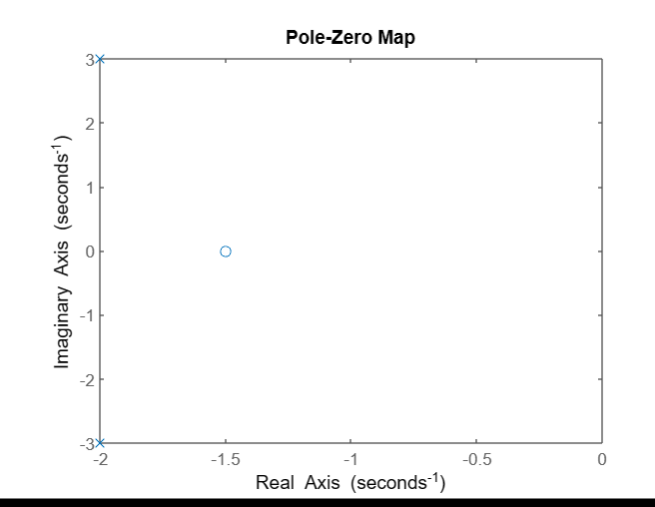
\includegraphics[width=\linewidth]{fig1.png}
  \label{fig:fig1}
\end{figure}


\subsubsection{Constructing transfer function from given zero pole:}
To construct transfer function from zeros \& poles ,we have to use zp2tf(z,p,k) and to print it in s form we have to use printsys() function

\begin{verbatim}
>> z=[4;2;-6];
>> p=[3;-64;9];
>> k = 10;
>> [n,d]=zp2tf(z,p,k);
>> printsys(n,d,'s')
 
num/den = 
 
       10 s^3 - 280 s + 480
   ---------------------------
   s^3 + 52 s^2 - 741 s + 1728
>> 
\end{verbatim}




\subsection{Response of a System Through Transfer Function:}
\subsubsection{impulse response:}
Say a differential equation be, 
\[2\frac{d^3y}{dt^3} + 44\frac{d^2y}{dt^2} +58 \frac{dy}{dt} + y = 34\frac{du}{dt} +29u\]
After transforming this into transfer function by “tf()” function ,the function “impulse()” will show its response.


\begin{lstlisting}[
frame = single,
numbers = left,
style = Matlab-Pyglike
]
n=[34 29]
d=[2 44 58 1];
G=tf(n,d)
impulse(G)
grid
\end{lstlisting}

\begin{verbatim}
>> n=[34 29]
>> d=[2 44 58 1];
>> G=tf(n,d)
>> impulse(G)
>> grid

n =

    34    29


G =
 
          34 s + 29
  -------------------------
  2 s^3 + 44 s^2 + 58 s + 1
 
Continuous-time transfer function.
\end{verbatim}



\begin{figure}[h!]
    \centering
    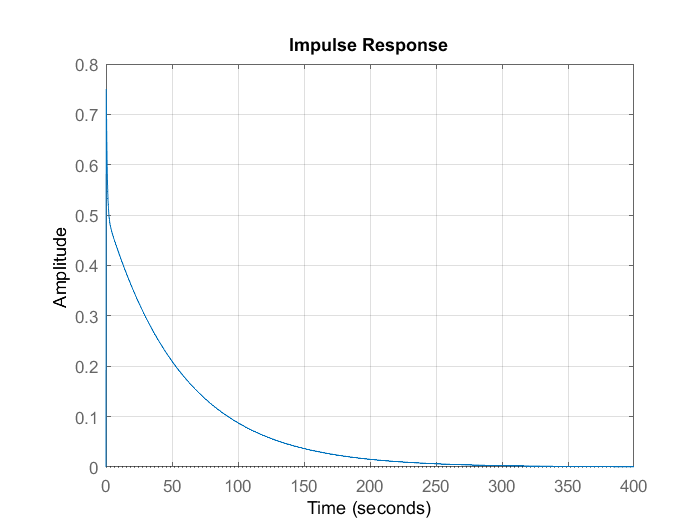
\includegraphics[width=\linewidth]{fig2.png}
    \label{fig:my_label}
\end{figure}



\subsubsection{ii)step response:}
\[2\frac{d^3y}{dt^3} + 44\frac{d^2y}{dt^2} +58 \frac{dy}{dt} + y = 34\frac{du}{dt} +29u\]
After transforming this into transfer function by “tf()” function ,the function “step()” will show its response.

\begin{verbatim}
>> n=[34 29]
>> d=[2 44 58 1];
>> G=tf(n,d)
>> step(G)
>> grid

n =

    34    29


G =
 
          34 s + 29
  -------------------------
  2 s^3 + 44 s^2 + 58 s + 1
 
Continuous-time transfer function.

>> 
\end{verbatim}

\begin{figure}[h!]
    \centering
    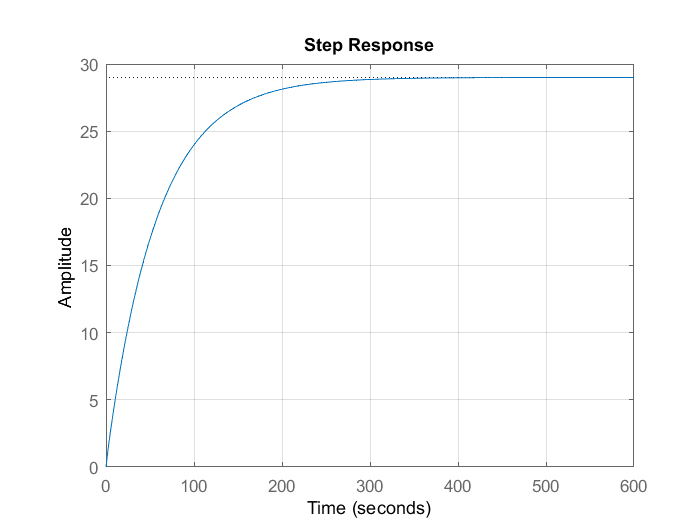
\includegraphics[width=\linewidth]{fig3.png}
    \label{fig:my_label}
\end{figure}


\subsubsection{Response to a general input}
Considering a transfer function given as
\begin{figure}[h!]
    \centering
    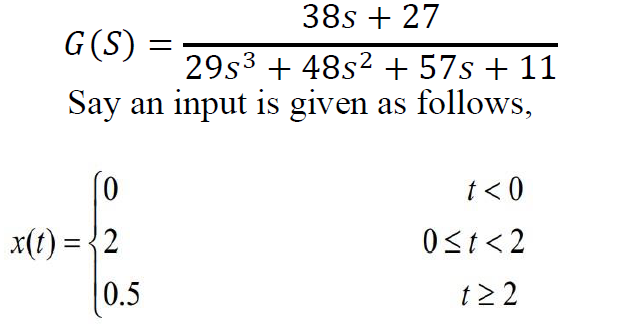
\includegraphics[width=\linewidth]{eq.png}
    \label{fig:my_label}
\end{figure}

for these inputs the response will be as follows
\begin{lstlisting}[
frame = single,
numbers = left,
style = Matlab-Pyglike
]
n=[38 27];
d=[29 48 57 11];
G=tf(n,d);
t1=0:0.02:2;
t2=2.02:0.02:10;
time=[t1 t2];
x=[2*ones(size(t1)) 0.5*ones(size(t2))];
y=lsim(G,x,time);
plot(time,y,time,x,'--');
gtext('input');
gtext('output');
\end{lstlisting}

\begin{verbatim}
>> n=[38 27];
>> d=[29 48 57 11];
>> G=tf(n,d);
>> t1=0:0.02:2;
>> t2=2.02:0.02:10;
>> time=[t1 t2];
>> x=[2*ones(size(t1)) 0.5*ones(size(t2))];
>> y=lsim(G,x,time);
>> plot(time,y,time,x,'--');
>> gtext('input');
>> gtext('output');
>> 
\end{verbatim}
\begin{figure}[h!]
  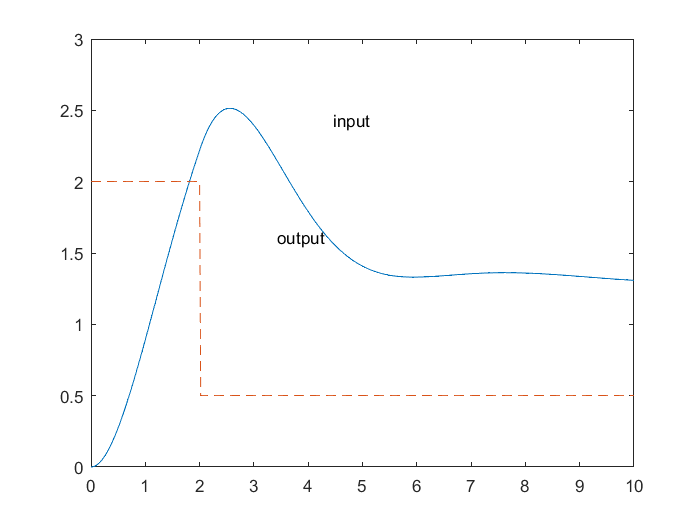
\includegraphics[width=\linewidth]{output.png}
  \label{fig:fig1}
\end{figure}

\subsection{Home Work:}
Q-1.1)Find the Laplace Transform of 
\[12\frac{d^2f}{dt^2}\]
Answer:
\begin{verbatim}
>> syms f(s);
>> df = 12 * (diff(f(s),2));
>> fs0 = laplace(df, 's')
 
fs0 =
 
12*s^2*laplace(f(s3), s3, s) - 12*s*f(0) - 12*subs(diff(f(s), s), s, 0)
 
>> 
\end{verbatim}
Q-1.2)Obtain the Laplace transform of the 
following f(t) using MATLAB.
$$ i)f(t) = e^{-3t} cos4t $$\\*
$$ii)f(t) = 1 - 2e^{-4t} + e^{-5t} $$
\hspace{5em}
Answer:
\begin{verbatim}
>> % i. f(t) = e^-3tcos4t
>> syms t;
>> ft = exp(-3*t)*(cos(4*t));
>> fs = laplace(ft)
 
fs =
 
(s + 3)/((s + 3)^2 + 16)
 
>> % f(t) = 1 - 2e-4t + e-5t
>> syms t;
>> ft = 1 - 2 *exp(-4*t) + exp(-5*t);
>> fs = laplace(ft)
 
fs =
 
1/(s + 5) - 2/(s + 4) + 1/s
 
>> 
\end{verbatim}



Q-1.3) Obtain the inverse Laplace transform of 
the following F(s).:
\begin{figure}[h!]
    \centering
    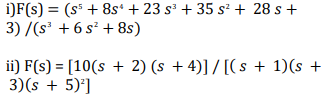
\includegraphics[width=\linewidth]{q1.3.png}
    \label{fig:my_label}
\end{figure}

\begin{lstlisting}[
frame=single,
numbers=left,
style=Matlab-Pyglike]
syms s t;
fs = (s^5 + 8 *s^4 + 23*s^3+35*s^2 + 28*s+3)/(s^3 + 6*s^2 + 8 * s) 
ft = ilaplace(fs)

\end{lstlisting}
\begin{verbatim}
fs =
 
(s^5 + 8*s^4 + 23*s^3 + 35*s^2 + 28*s + 3)/(s^3 + 6*s^2 + 8*s)
 
 
ft =
 
exp(-2*t)/4 + (3*exp(-4*t))/8 + 3*dirac(t) + 2*dirac(1, t) + dirac(2, t) + 3/8
\end{verbatim}
Q-1.4)Given the zeros, poles and gain K of 
B(s)/A(s). Obtain the function B(s)/A(s) :\\
1)There is no zero. Poles are at -1 + 2j and −1 −
2j and K = 10. \\
2) A zero is at −1. Poles are at −2, −4 and −8. K = 
12\\
3) Zeros are at −1 and −2. Poles are at 0, −4 and 
−6. K = 5.\\
4) A zero is at 0. Poles are at -1 + 2j and −1 − 2j. 
K = 10.


\begin{verbatim}
    %solution (i)
    >> z = [];
>> p = [-1 + 2j; -1-2j];
>> k = 10;
>> [n, d] = zp2tf(z,p, k);
>> printsys(n,d,'s')
 
num/den = 
 
         10
   -------------
   s^2 + 2 s + 5

>> %soln (ii)
>> z = [-1];
>> p = [-2;-4;-8];
>> k = 12;
>> [n, d] = zp2tf(z,p, k);
>> printsys(n,d,'s')
 
num/den = 
 
           12 s + 12
   ------------------------
   s^3 + 14 s^2 + 56 s + 64
>> % solution (iii)
>> z = [-1; -2];
>> p = [0;-4;-6]












p =

     0
    -4
    -6

>> k = 5;
>> [n, d] = zp2tf(z,p, k);
>> printsys(n,d,'s')
 
num/den = 
 
    5 s^2 + 15 s + 10
   -------------------
   s^3 + 10 s^2 + 24 s
>> solution(iv)
>> z = [0];
>> p = [-1+2j; -1-2j];
>> k=10;
>> [n,d] = zp2tf(z,p,k);
>> printsys(n,d,'s')
 
num/den = 
 
        10 s
   -------------
   s^2 + 2 s + 5
>> 
\end{verbatim}
Q-1.5)Find the transfer Function of the 
following system
\begin{figure}[h!]
    \centering
    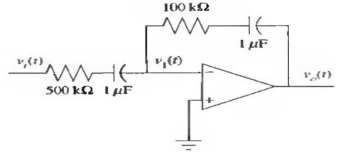
\includegraphics[width=\linewidth]{system.png}
    \label{fig:my_label}
\end{figure}

Answer:
As the given Op-amp circuit represents an 
inverter circuit,so the the transfer function 
of this circuit can be defined as,
\[G(s) =    \frac{V_output}{V_input} =\frac{v_o}{v_i} = \frac{-z_2}{z_1}\]

We know, 
        \[z_1 = R_1 + X_{c_{2}}\] 
        \[z_2 = R_2 + X_{c_{2}}\]

Given,
\[R_1 = 5*10^5 \Omega\] \\
\[R_2 = 10^6 \Omega\]
So,
\[X_{c_{1}} =\frac{1}{1uFx S}= \frac{1}{SC} =\frac{1}{10^{-6} x S} = X_{c_{2}}\]

\[z_1 = \frac{0.5s +1}{10^{-6}}\] \\
\[z_2 = \frac{0.1s +1 }{10^{-6}}\]
Therefore, the transfer function is
\begin{figure}[!h]
    \centering
    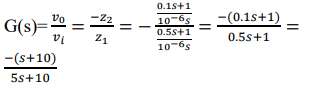
\includegraphics[width =\linewidth]{transff.PNG}
    \label{fig:my_label}
\end{figure}


Q-1.6) Obtain a plot of the ramp response 
of the system whose transfer function is 
shown below:
\[G(s) = \frac{3s + 2}{2s^3 + 4s^2 + 5s + 1}\]
Solution:
\begin{lstlisting}[
frame = single,
numbers = left,
style=Matlab-Pyglike
]
% G(s) = 3s + 2/2s^3  + 4s^2+5s+1
n = [3 2];
d = [2 4 5 1];
G = tf(n,d)
\end{lstlisting}
\begin{verbatim}
>> % G(s) = 3s + 2/2s^3  + 4s^2+5s+1
>> n = [3 2];
>> d = [2 4 5 1];
>> G = tf(n,d)

G =
 
          3 s + 2
  -----------------------
  2 s^3 + 4 s^2 + 5 s + 1
 
Continuous-time transfer function.

>> t = 0:0.02:10;
>> time = [t];
>> x = [t.*ones(size(t))];
>> y = lsim(G,x,time);
>> plot(time, y, time, x, '--')
>> gtext('input')
>> gtext('output')
\end{verbatim}


Output Diagram:


\begin{figure}[!h]
    \centering
    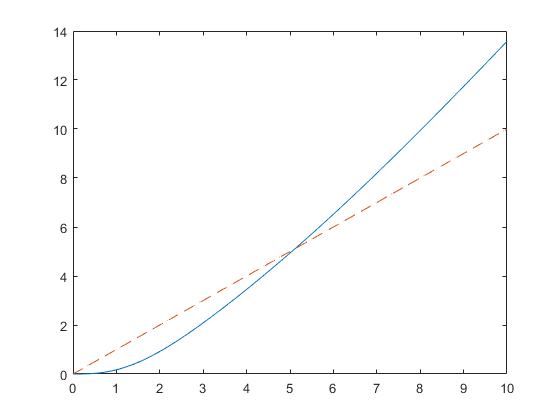
\includegraphics[width=\linewidth]{plot1.png}
    \label{fig:my_label}
\end{figure}


\section{Discussion:}
In this experimentaion and analysis we have 
learnt to handle polynomials in MATLAB.We 
have observed laplace and inverse 
laplace transformation in MATLAB 
command. We learnt to determine pole 
\& zeros and also learn to show them in pole zero 
map. We observed responses 
for various input signals through this experimentation.



\end{document}
